\documentclass[12pt]{article}
\usepackage{amsmath}
\usepackage{amssymb}
\usepackage{enumerate}
\usepackage{geometry}
\usepackage{tikz}
\usetikzlibrary{automata, positioning, arrows}
\geometry{margin=1in}

\title{Homework 2 - CPSC 326\\Solutions}
\author{Dang Phung}
\date{September 30th, 2025}

\begin{document}
\maketitle

\section*{Question 1 (10 points)}
Let $\Sigma = \{0, 1\}$. Let $L_1 = \{w \in \Sigma^* \mid |w|_0 \neq |w|_1\}$. Prove or disprove that $L_1^* = \Sigma^*$.

\textbf{Answer:}

We will \textbf{prove} that $L_1^* = \Sigma^*$.

To show $L_1^* = \Sigma^*$, we need to show that every string in $\Sigma^*$ can be shown  as a concatenation of strings from $L_1$.

First off,
\begin{itemize}
    \item $0 \in L_1$ since $|0|_0 = 1 \neq 0 = |0|_1$
    \item $1 \in L_1$ since $|1|_1 = 1 \neq 0 = |1|_0$
    \item $\lambda \in L_1^*$ since $L_1^0 = \{\lambda\}$
\end{itemize}

For any non-empty string $w \in \Sigma^*$, you can write it as $w = \sigma_1\sigma_2\cdots\sigma_n$ where each $\sigma_i \in \{0, 1\}$.

Since each single symbol ($0$ or $1$) is in $L_1$, we have:
$$w = \sigma_1 \cdot \sigma_2 \cdot \ldots \cdot \sigma_n \in L_1^n \subseteq L_1^*$$

Therefore, every string in $\Sigma^*$ including $\lambda$ is in $L_1^*$.

This gives us $\Sigma^* \subseteq L_1^*$. Since $L_1^* \subseteq \Sigma^*$ by definition, we prove that
$$L_1^* = \Sigma^*$$

\section*{Question 2 (10 points)}
Let $L_2 = \{w \in \{1, 2, 3\}^* \mid |w| \bmod 2 = 0\}$. Given the linear ordering $1 < 2 < 3$ on $\Sigma$, list the first 10 elements, in canonical order, in an enumeration of $L_2$.

\textbf{Answer:}

Canonical order means: order by length, and then lexicographically within each length.

$L_2$ contains all strings of even length over $\{1, 2, 3\}$ (mod 2  = 0).

\textbf{First 10 elements:}
\begin{enumerate}
    \item $\lambda$
    \item $11$
    \item $12$
    \item $13$
    \item $21$
    \item $22$
    \item $23$
    \item $31$
    \item $32$
    \item $33$
\end{enumerate}

\section*{Question 3 (10 points)}
Design a DFA for the following regular language:
$$L_3 = \{w \in \{a, b, c, 1, 2\}^* \mid w \text{ does not contain the substring } 1a1\}$$

\textbf{Answer:}


\begin{center}
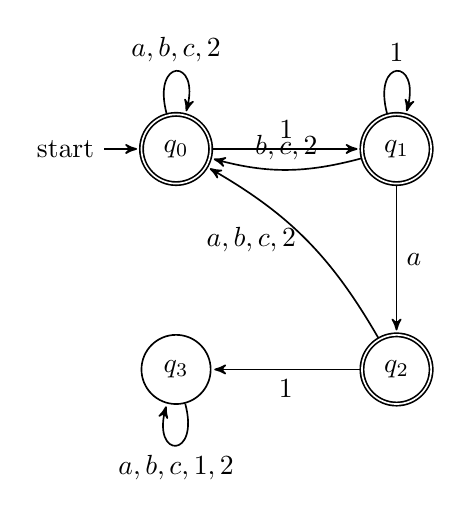
\begin{tikzpicture}[>=stealth', shorten >=1pt, auto, node distance=2.8cm, semithick]
    \node[state, initial, accepting] (q0) {$q_0$};
    \node[state, accepting] (q1) [right of=q0] {$q_1$};
    \node[state, accepting] (q2) [below of=q1] {$q_2$};
    \node[state] (q3) [below of=q0] {$q_3$};
    
    \path[->]
    (q0) edge node {$1$} (q1)
    (q0) edge [loop above] node {$a,b,c,2$} (q0)
    (q1) edge [loop above] node {$1$} (q1)
    (q1) edge node {$a$} (q2)
    (q1) edge [bend left=15] node [above] {$b,c,2$} (q0)
    (q2) edge node {$1$} (q3)
    (q2) edge [bend right=15] node [left] {$a,b,c,2$} (q0)
    (q3) edge [loop below] node {$a,b,c,1,2$} (q3);
\end{tikzpicture}
\end{center}

\section*{Question 4 (10 points)}
Design a DFA for the following regular language:
$$L_4 = \{w \in \{a, b, c, 1, 2\}^* \mid w \text{ contains the substring } 1a1\}$$

\textbf{Answer:}

\begin{center}
\begin{tikzpicture}[>=stealth', shorten >=1pt, auto, node distance=2.8cm, semithick]
    \node[state, initial] (q0) {$q_0$};
    \node[state] (q1) [right of=q0] {$q_1$};
    \node[state] (q2) [below of=q1] {$q_2$};
    \node[state, accepting] (qa) [below of=q0] {$q_a$};
    
    \path[->]
    (q0) edge node {$1$} (q1)
    (q0) edge [loop above] node {$a,b,c,2$} (q0)
    (q1) edge [loop above] node {$1$} (q1)
    (q1) edge node {$a$} (q2)
    (q1) edge [bend left=15] node [above] {$b,c,2$} (q0)
    (q2) edge node {$1$} (q3)
    (q2) edge [bend right=15] node [left] {$a,b,c,2$} (q0)
    (q3) edge [loop below] node {$a,b,c,1,2$} (q3);
\end{tikzpicture}
\end{center}

\section*{Question 5 (10 points)}
Design a DFA for the following regular language:
$$L_5 = \{w \in \{a, b, c\}^* \mid |w| \bmod 3 = 0\}$$

\textbf{Answer:}

\begin{center}
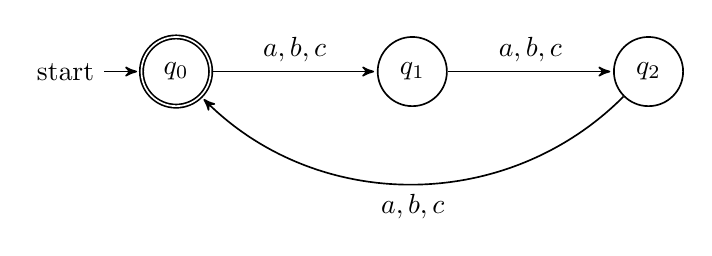
\begin{tikzpicture}[>=stealth', shorten >=1pt, auto, node distance=3cm, semithick]
    \node[state, initial, accepting] (q0) {$q_0$};
    \node[state] (q1) [right of=q0] {$q_1$};
    \node[state] (q2) [right of=q1] {$q_2$};
    
    \path[->]
    (q0) edge node {$a,b,c$} (q1)
    (q1) edge node {$a,b,c$} (q2)
    (q2) edge [bend left=45] node [below] {$a,b,c$} (q0);
\end{tikzpicture}
\end{center}

\section*{Question 6 (10 points)}
Design a DFA for the following regular language:
$$L_6 = \{w \in \{a, b, c\}^* \mid |w|_a \bmod 2 = 0 \text{ and } |w|_b \bmod 2 = 0\}$$

\textbf{Answer:}

\begin{center}
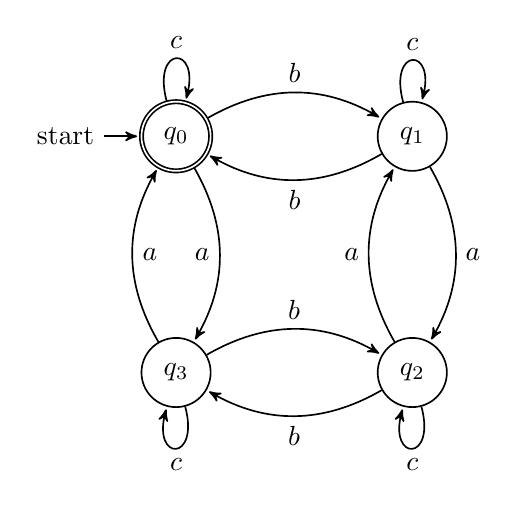
\begin{tikzpicture}[>=stealth', shorten >=1pt, auto, node distance=3cm, semithick]
    \node[state, initial, accepting] (q0) {$q_{0}$};
    \node[state] (q1) [right of=q0] {$q_{1}$};
    \node[state] (q3) [below of=q0] {$q_{3}$};
    \node[state] (q2) [right of=q3] {$q_{2}$};
    
    \path[->]
    (q0) edge [bend left] node {$b$} (q1)
    (q1) edge [bend left] node {$b$} (q0)
    (q0) edge [bend left] node [left] {$a$} (q3)
    (q3) edge [bend left] node [right] {$a$} (q0)
    (q1) edge [bend left] node [right] {$a$} (q2)
    (q2) edge [bend left] node [left] {$a$} (q1)
    (q3) edge [bend left] node {$b$} (q2)
    (q2) edge [bend left] node {$b$} (q3)
    (q0) edge [loop above] node {$c$} (q0)
    (q1) edge [loop above] node {$c$} (q1)
    (q3) edge [loop below] node {$c$} (q3)
    (q2) edge [loop below] node {$c$} (q2);
\end{tikzpicture}
\end{center}

\section*{Question 7 (10 points)}
Design a DFA for the following regular language:
$$L_7 = \{w \in \{a, b\}^* \mid \text{length of } w \text{ is even and } w \text{ contains the substring } aa\}$$

\textbf{Answer:}

\begin{center}
    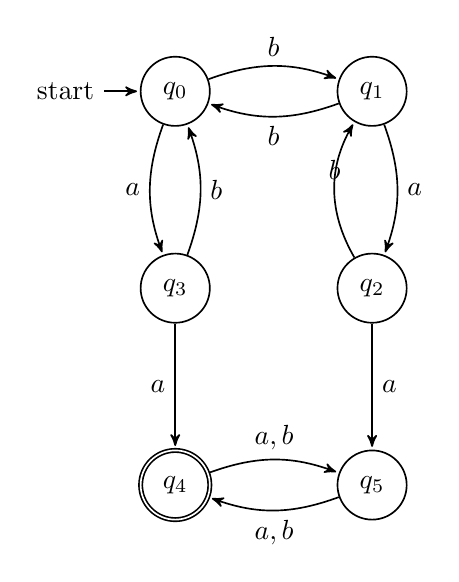
\begin{tikzpicture}[>=stealth', shorten >=1pt, auto, node distance=2.5cm, semithick]
        \node[state, initial] (q0) {$q_0$};
        \node[state] (q1) [right of=q0] {$q_1$};
        \node[state] (q2) [below of=q1] {$q_2$};
        \node[state] (q3) [below of=q0] {$q_3$};
        \node[state, accepting] (q4) [below of=q3] {$q_4$};
        \node[state] (q5) [right of=q4] {$q_5$};
        
        \path[->]
        (q0) edge [bend left=20] node [above] {$b$} (q1)
        (q1) edge [bend left=20] node [below] {$b$} (q0)
        (q0) edge [bend right=20] node [left] {$a$} (q3)
        (q3) edge [bend right=20] node [right] {$b$} (q0)
        (q1) edge [bend left=20] node [right] {$a$} (q2)
        (q2) edge [bend left=30] node [above] {$b$} (q1)
        (q2) edge node [right] {$a$} (q5)
        (q3) edge node [left] {$a$} (q4)
        (q4) edge [bend left=20] node [above] {$a,b$} (q5)
        (q5) edge [bend left=20] node [below] {$a,b$} (q4);
    \end{tikzpicture}
    \end{center}

\section*{Question 8 (10 points)}
Design a DFA for the following regular language:
$$L_8 = \{w \in \Sigma_{\text{bool}}^* \mid w \text{ contains at least one '0' and an even number of 1s following the last 0}\}$$

\textbf{Answer:}

\begin{center}
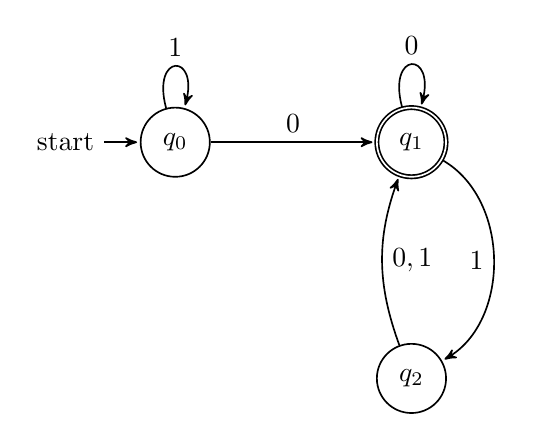
\begin{tikzpicture}[>=stealth', shorten >=1pt, auto, node distance=3cm, semithick]
    \node[state, initial] (q0) {$q_0$};
    \node[state, accepting] (q1) [right of=q0] {$q_1$};
    \node[state] (q2) [below of=q1] {$q_2$};
    
    \path[->]
    (q0) edge [loop above] node {$1$} (q0)
    (q0) edge node {$0$} (q1)
    (q1) edge [loop above] node {$0$} (q1)
    (q1) edge [bend left=60] node [left] {$1$} (q2)
    (q2) edge [bend left=20] node [right] {$0,1$} (q1);
\end{tikzpicture}
\end{center}

\section*{Question 9 (10 points)}
Design a DFA for the following regular language:
$$L_9 = \{w \in \{a, b, c\}^* \mid \text{Every fourth symbol of } w \text{ is a 'b'}\}$$

\textbf{Answer:}

\begin{center}
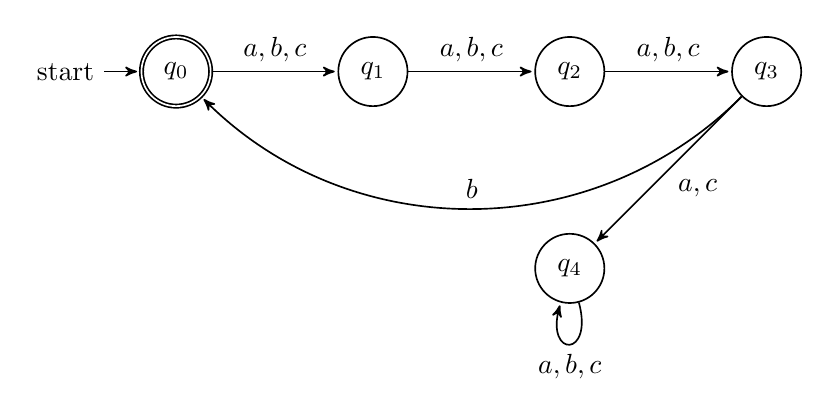
\begin{tikzpicture}[>=stealth', shorten >=1pt, auto, node distance=2.5cm, semithick]
    \node[state, initial, accepting] (q0) {$q_0$};
    \node[state] (q1) [right of=q0] {$q_1$};
    \node[state] (q2) [right of=q1] {$q_2$};
    \node[state] (q3) [right of=q2] {$q_3$};
    \node[state] (q4) [below of=q2] {$q_4$};
    
    \path[->]
    (q0) edge node {$a,b,c$} (q1)
    (q1) edge node {$a,b,c$} (q2)
    (q2) edge node {$a,b,c$} (q3)
    (q3) edge [bend left=45] node [above] {$b$} (q0)
    (q3) edge node {$a,c$} (q4)
    (q4) edge [loop below] node {$a,b,c$} (q4);
\end{tikzpicture}
\end{center}

\section*{Question 10 (10 points)}
Design a DFA for the following regular language:
$$L_{10} = \{w \in \{a, b, c, 1, 2\}^* \mid w \text{ does not contain } 1b2a\}$$

\textbf{Answer:}

\begin{center}
    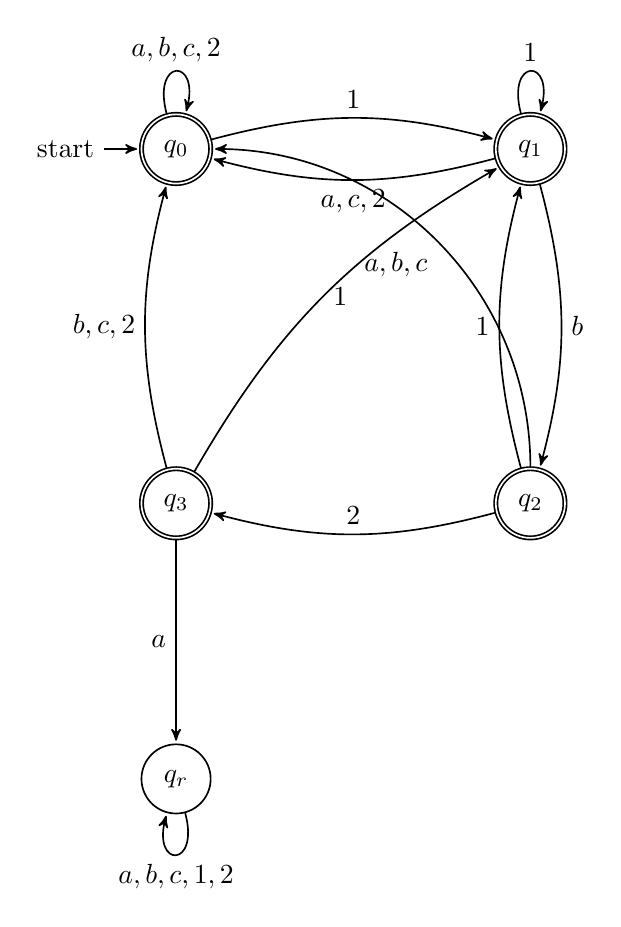
\begin{tikzpicture}[>=stealth', shorten >=1pt, auto, node distance=4.5cm, semithick]
        \node[state, initial, accepting] (q0) {$q_0$};
        \node[state, accepting] (q1) [right of=q0] {$q_1$};
        \node[state, accepting] (q2) [below of=q1] {$q_2$};
        \node[state, accepting] (q3) [below of=q0] {$q_3$};
        \node[state] (qr) [below of=q3, node distance=3.5cm] {$q_r$};
        
        \path[->]
        (q0) edge [bend left=15] node [above] {$1$} (q1)
        (q0) edge [loop above] node {$a,b,c,2$} (q0)
        (q1) edge [loop above] node {$1$} (q1)
        (q1) edge [bend left=15] node [right] {$b$} (q2)
        (q1) edge [bend left=15] node [below] {$a,c,2$} (q0)
        (q2) edge [bend left=15] node [left] {$1$} (q1)
        (q2) edge [bend left=15] node [above] {$2$} (q3)
        (q2) edge [bend right=45] node [below left] {$a,b,c$} (q0)
        (q3) edge [bend left=15] node [right] {$1$} (q1)
        (q3) edge node [left] {$a$} (qr)
        (q3) edge [bend left=15] node [left] {$b,c,2$} (q0)
        (qr) edge [loop below] node {$a,b,c,1,2$} (qr);
    \end{tikzpicture}
    \end{center}


\end{document}